\section{Method}
\subsection{Participants}
The study has been approved by the PaLS - Institute of Cognitive Neuroscience/ BUCNI LREC as Project ID 0210. For the acquaintance group, 17 interconnected participants who provided their laughter recordings in 2012 were contacted again, and 10 of them responded and completed the experiment. Seven additional family members/friends of these laughers were recruited through a snowball sampling technique (referred by laughers). The final acquaintance group of 17 participants consisted of 10 females and 7 males, between the ages of 18 and 61 (\textit{M }= 41.29, \textit{SD} = 16.81).

\subsection{Materials}
The experiment was built and conducted on the Gorilla (https://gorilla.sc/), an online experiment builder platform \citep {anwyl2020gorilla}. Participants completed the task on their personal computers and headphones.

\subsubsection{Laughter Perception Task (LPT)}

LPT consisted of two blocks. Both blocks involved listening to recordings of laughter. 68 spontaneous laughter recordings were collected from 17 laughers (7 females and 10 males) in 2012. While these participants were shown funny YouTube videos, their natural responses were recorded in an Anechoic chamber. Each laugher contributed two recordings per block.

In Block 1, participants were not informed of the names of laughers in the recording. After listening to each recording, they were asked to 1) rate the contagion (“How much does this laughter make you laugh”) on a scale from 1, meaning “I don’t want to laugh at all,” to 10 “I laugh a lot.” 2) rate the familiarity (“does this laughter sound familiar?”) on a scale from 1, meaning “not familiar,” to 10, “very familiar” (Figure 1). In order to ensure participants focused on the task, three vigilance trials were also applied in random order, in which participants were asked to select the number that the speaker in the audio said. A total of 37 trials ( 34 laughter perception trials and 3 vigilance trials) were conducted.

In Block 2, before listening to the laughter recording, participants in the acquaintance group were presented with the laugher’s name, a manipulation reffered to as the informing effect. After listening to each recording, they were again asked to rate the contagiousness of laughter on the same scale as above. Differently, this time, they were asked to judge their closeness with the laugher (“Is this person close to you?”) instead of familiarity, on a scale from 1 “not close” to 10 “very close” (see Figure~\ref{fig:block}). Three vigilance trials were applied. A total of 37 trials ( 34 laughter perception trials and 3 vigilance trials) were conducted.

\begin{figure}[h!] 
\centering
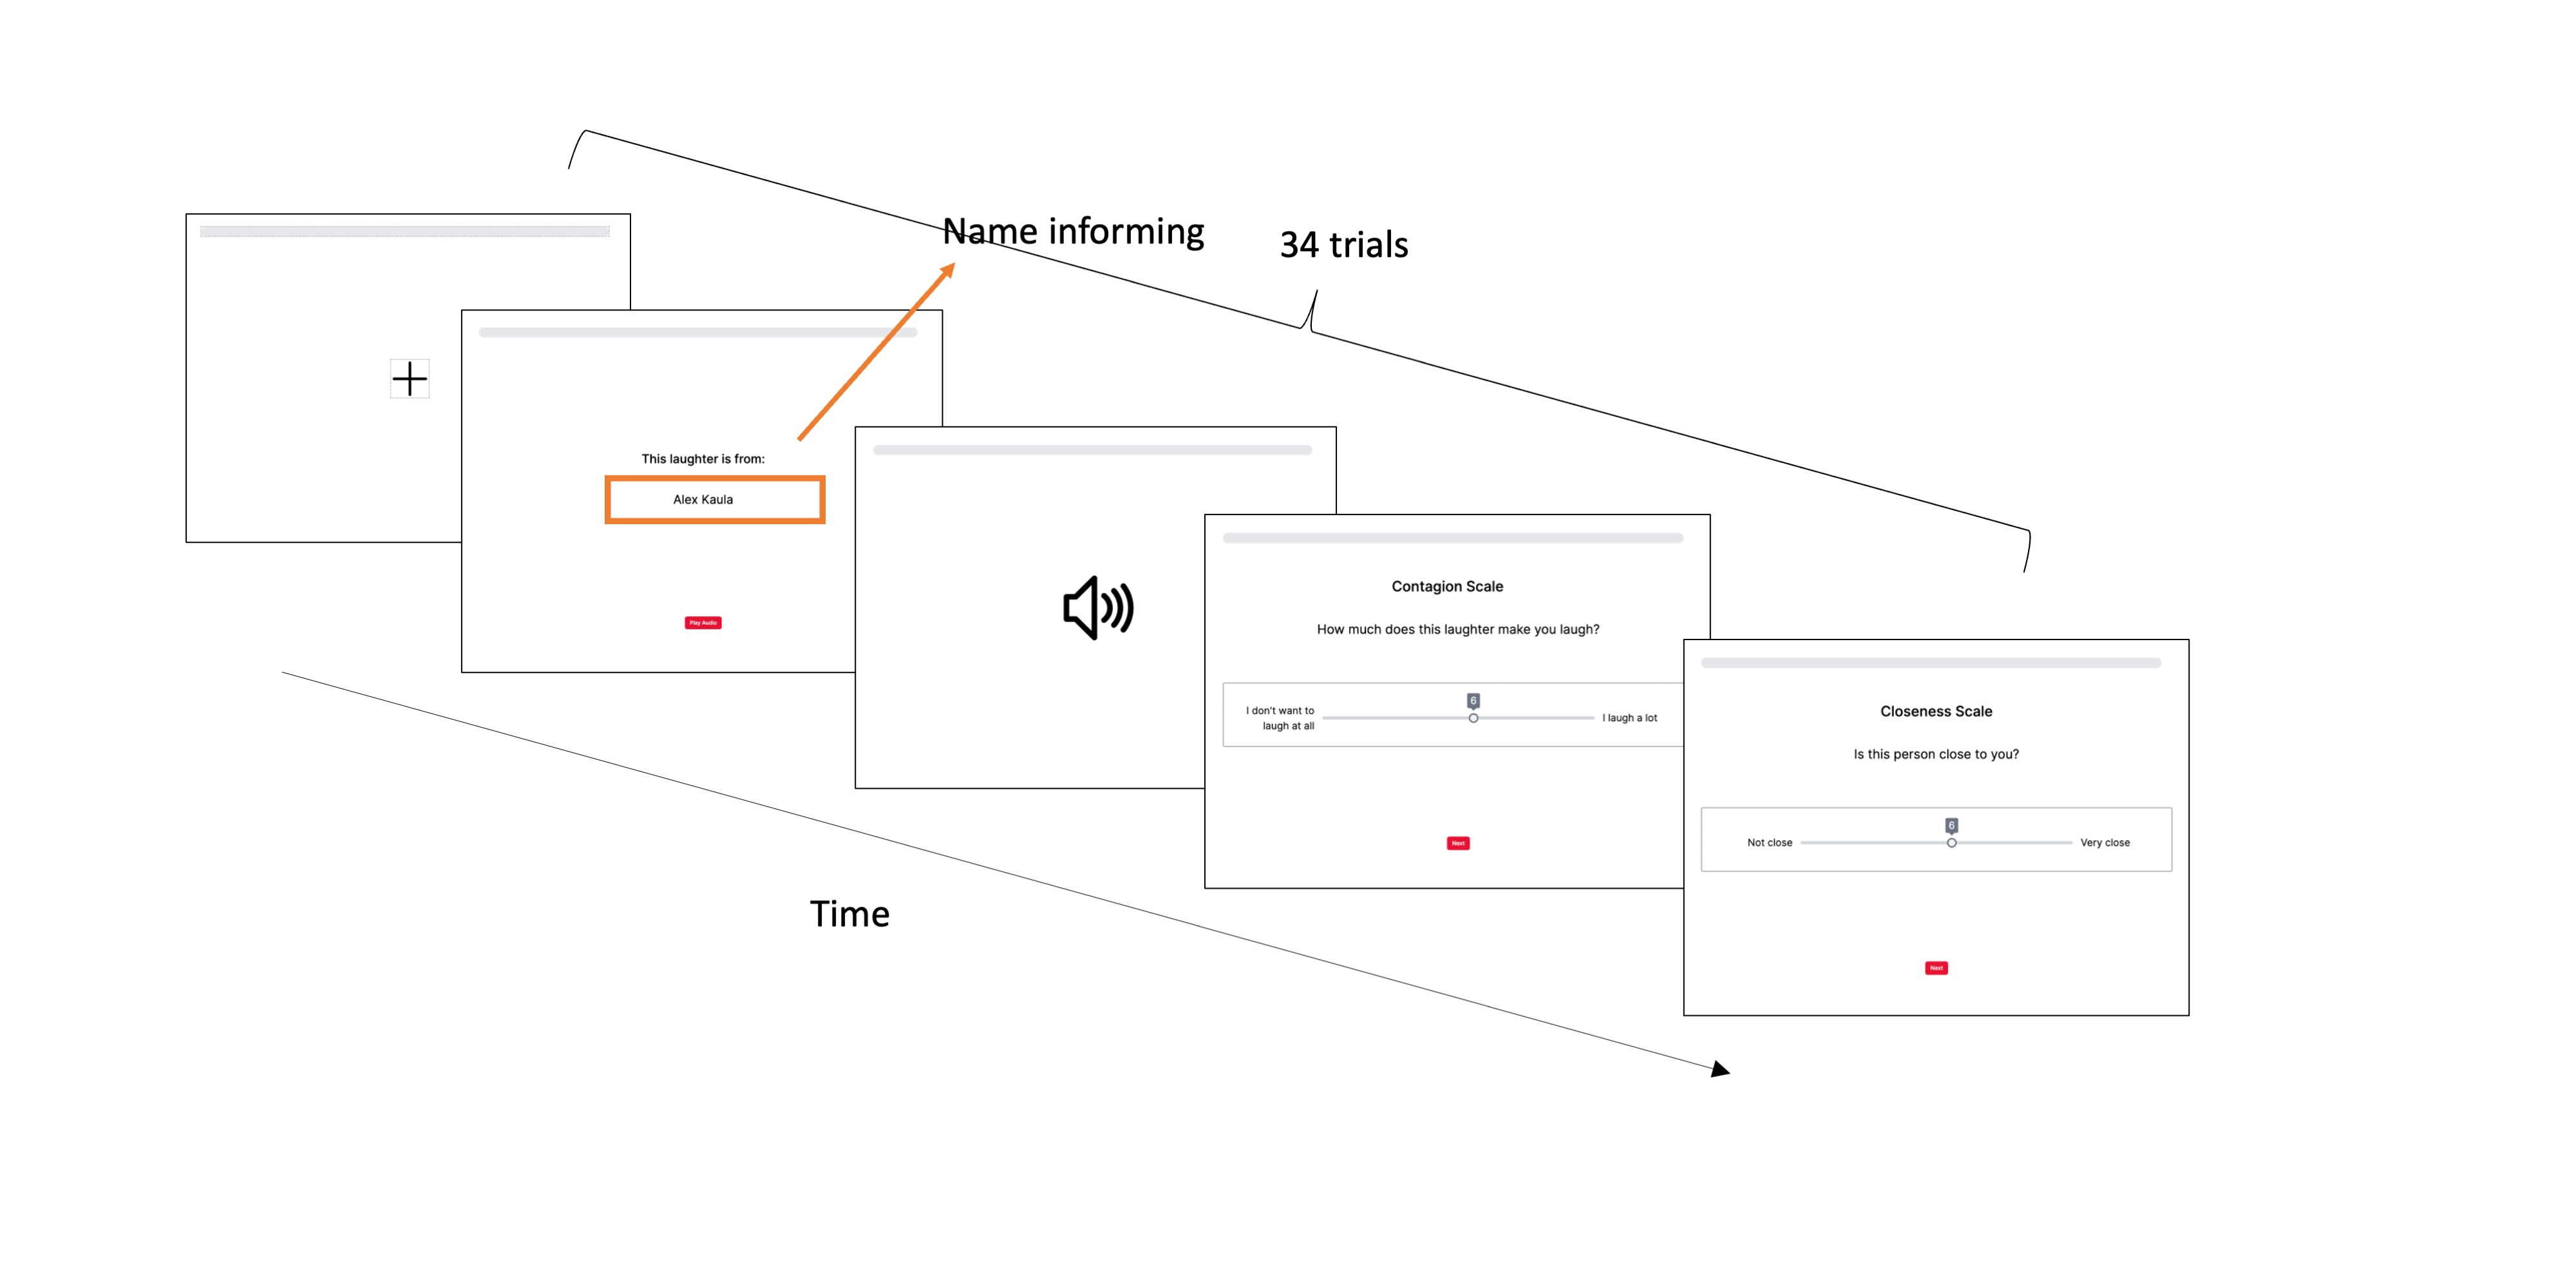
\includegraphics[width=1\textwidth]{Slide2.jpeg}
\caption{\label{fig:block}This is a another figure caption.}
\end{figure}

\subsection{Procedure}
The order of the experiment is shown in Figure 3. Participants in the acquaintance group were invited to the Gorilla online experiment through an email link; the stranger group was invited through Prolific. After providing informed consent, participants completed a sound check to ensure the audio devices were connected.

Participants were first asked to provide demographic information (age, gender, sex) and then completed two questionnaires (LSAS and LPPQ).

